\section{Aplicación} 

\subsection{Las diferencias entre Business Intelligence y Business Analytics}

Inteligencia de Negocios (BI)y Business Analytics son similares, aunque no son exactamente iguales. Business Intelligence implica el proceso de recopilación de datos de todas las fuentes y su preparación para Business Analytics. Business Intelligence es más un primer paso que las empresas deben tomar cuando necesitan la capacidad de tomar decisiones basadas en datos.\newline

Business Analytics, por otro lado, es el análisis de las respuestas proporcionadas por Business Intelligence. Mientras que Business Intelligence responde lo que sucedió, Business Analytics responde por qué sucedió y si volverá a suceder.\newline

Business Intelligence incluye:

\begin{itemize}
\item Informes.
\item Supervisión y alertas automatizadas.
\item Paneles de control.
\item Cuadros de mandos.
\item Consultas ad hoc (una solución elaborada específicamente para un problema).\newline
\end{itemize}

Business Analytics, en contraste, incluye:

\begin{itemize}
\item Análisis estadístico y cuantitativo.
\item Minería de datos.
\item Modelos predictivos.
\item Pruebas multivariable.\newline
\end{itemize}

\begin{center}
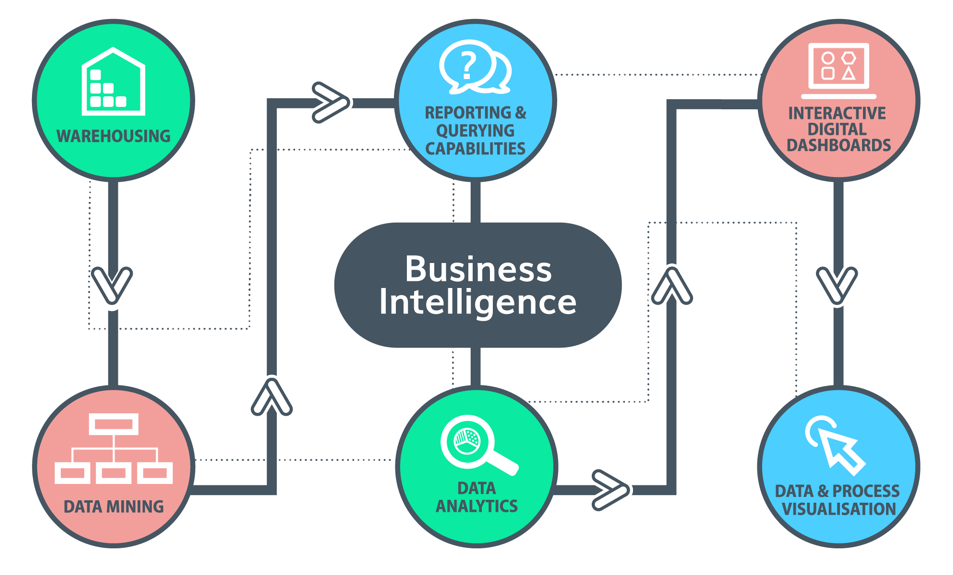
\includegraphics[width=0.6\columnwidth]{images/bi/bi-t}\newline
\end{center}